\chapter{Entwurf}
\section{Pakete}
Unsere Software gliedert sich in drei Pakete, deren Struktur in Abbildung \ref{Paketdiagramm} dargestellt ist.

%Paketdiagramm
\begin{figure}[H]
	\centering
	%\hspace{-.5cm}
	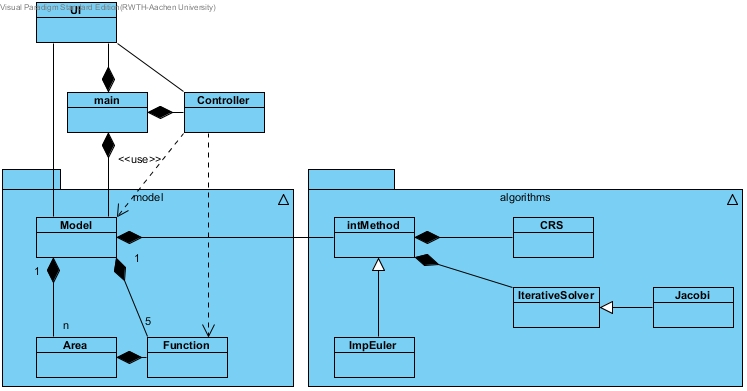
\includegraphics[scale=.65]{Bilder/Paketdiagramm.jpg}\\
	\caption{Paketstruktur}
	\label{Paketdiagramm}
\end{figure}

\section{Abstrakte Datentypen}

\section{Klassen}

Nachfolgend sind die Klassen-/Sequenzdiagramme nach Paketen sortiert aufgelistet. \\
Dabei werden keine Sequenzdiagramme gezeigt, falls es sich um Methoden ohne Kommunikation mit anderen Objekten handelt, insbesondere auch getter-Funktionen oder Funktionen die Algorithmen implementieren.

\subsection{Paket algorithms}

Das Klassendiagramm in Abbildung \ref{Klassendiagramm algorithms} zeigt alle im Paket \emph{algorithms} enthaltene Klassen.

%Klassendiagramm algorithms
\begin{figure}[H]
	\centering
	%\hspace{-.5cm}
	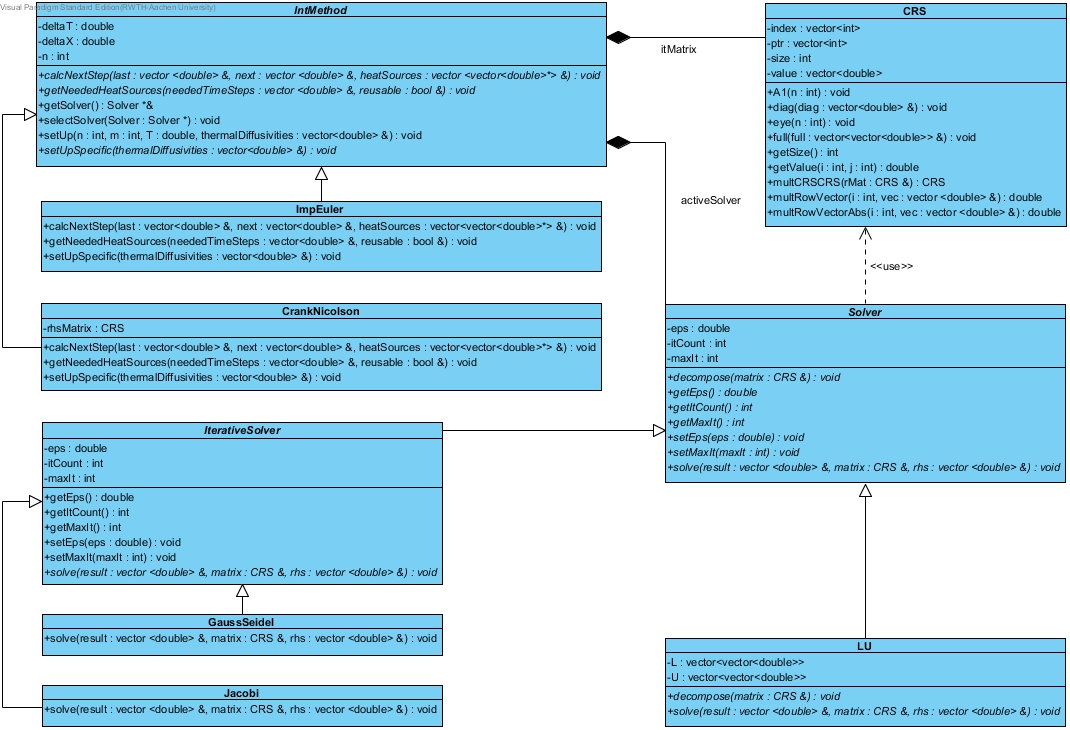
\includegraphics[scale=.52]{Bilder/algorithms.jpg}\\
	\caption{Klassendiagramm algorithms}
	\label{Klassendiagramm algorithms}
\end{figure}

\subsubsection{IntMethod}

\subsubsection*{calcNextStep}

Das Sequenzdiagramm für \emph{calcNextStep} ist in Abbildung \ref{Sequenzdiagramm calcNextStep} dargestellt. \emph{calcNextStep} berechnet die Approximation der Temperaturverteilung zum nächsten Zeitpunkt unter Verwendung der aktuellen Verteilung sowie der eingegebenen Temperaturleitkoeffizienten und Wärmequellen.

%Sequenzdiagramm calcNextStep
\begin{figure}[H]
	\centering
	%\hspace{-.5cm}
	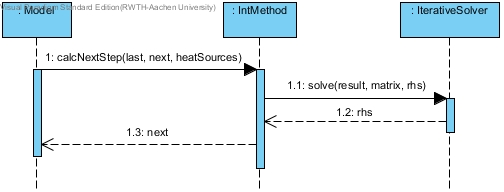
\includegraphics[scale=.6]{Bilder/IntMethod__calcNextStep().jpg}\\
	\caption{Sequenzdiagramm calcNextStep}
	\label{Sequenzdiagramm calcNextStep}
\end{figure}

\subsubsection*{selectSolver}

Das Sequenzdiagramm für \emph{selectSolver} ist in  Abbildung \ref{Sequenzdiagramm selectSolverIntMethod} dargestellt.
\emph{selectSolver} setzt den gewählten Löser für lineare Gleichungssysteme.

%Sequenzdiagramm selectSolver
\begin{figure}[H]
	\centering
	%\hspace{-.5cm}
	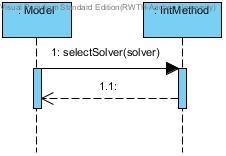
\includegraphics{Bilder/IntMethod__selectSolver().jpg}\\
	\caption{Sequenzdiagramm selectSolver}
	\label{Sequenzdiagramm selectSolverIntMethod}
\end{figure}

\subsubsection*{setUp}

Das Sequenzdiagramm für \emph{setUp} ist in  Abbildung \ref{Sequenzdiagramm setUp} dargestellt. \emph{setUp} bereitet die Simulationsberechnung vor.

%Sequenzdiagramm setUp
\begin{figure}[H]
	\centering
	%\hspace{-.5cm}
	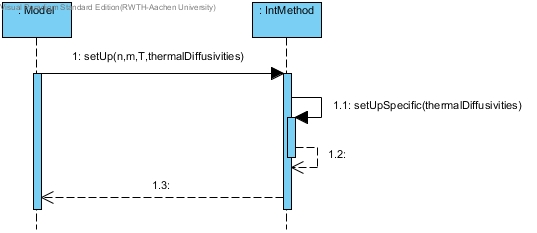
\includegraphics[scale=.6]{Bilder/IntMethod__setUp().jpg}\\
	\caption{Sequenzdiagramm setUp}
	\label{Sequenzdiagramm setUp}
\end{figure}

\subsubsection*{setUpSpecific}

Das Sequenzdiagramm für \emph{setUpSpecific} ist in Abbildung \ref{Sequenzdiagramm setUpSpecific} dargestellt. \emph{setUpSpecific} trifft für die gewählte Integrationsmethode spezifische Vorbereitungen.

%Sequenzdiagramm setUpSpecific
\begin{figure}[H]
	\centering
	%\hspace{-.5cm}
	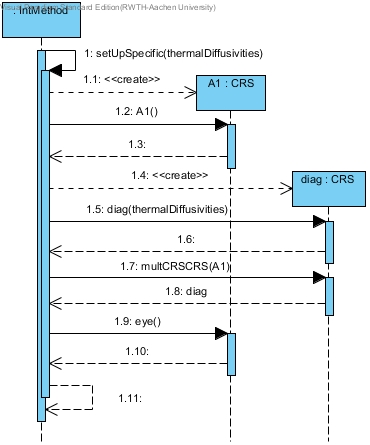
\includegraphics[scale=.6]{Bilder/IntMethod__setUpSpecific().jpg}\\
	\caption{Sequenzdiagramm setUpSpecific}
	\label{Sequenzdiagramm setUpSpecific}
\end{figure}

\subsubsection{IterativeSolver}

\subsubsection*{setEps}

Das Sequenzdiagramm für \emph{setEps} ist in  Abbildung \ref{Sequenzdiagramm setEps} dargestellt. \emph{setEps} setzt die gewählte relative Genauigkeit.

%Sequenzdiagramm setEps
\begin{figure}[H]
	\centering
	%\hspace{-.5cm}
	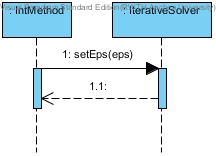
\includegraphics{Bilder/IterativeSolver__setEps().jpg}\\
	\caption{Sequenzdiagramm setEps}
	\label{Sequenzdiagramm setEps}
\end{figure}

\subsubsection*{setMaxIt}

Das Sequenzdiagramm für \emph{setMaxIt} ist in \ref{Sequenzdiagramm setMaxIt} dargstellt. \emph{setMaxIt} setzt die gewählte maximale Iterationsanzahl.

%Sequenzdiagramm setMaxIt
\begin{figure}[H]
	\centering
	%\hspace{-.5cm}
	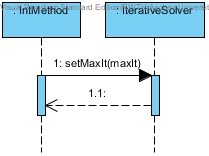
\includegraphics{Bilder/IterativeSolver__setMaxIt().jpg}\\
	\caption{Sequenzdiagramm setMaxIt}
	\label{Sequenzdiagramm setMaxIt}
\end{figure}

\subsection{Paket model}

Das Klassendiagramm in Abbildung \ref{Klassendiagramm model} zeigt alle im Paket \emph{model} enthaltene Klassen.

%Klassendiagramm model
\begin{figure}[H]
	\centering
	%\hspace{-.5cm}
	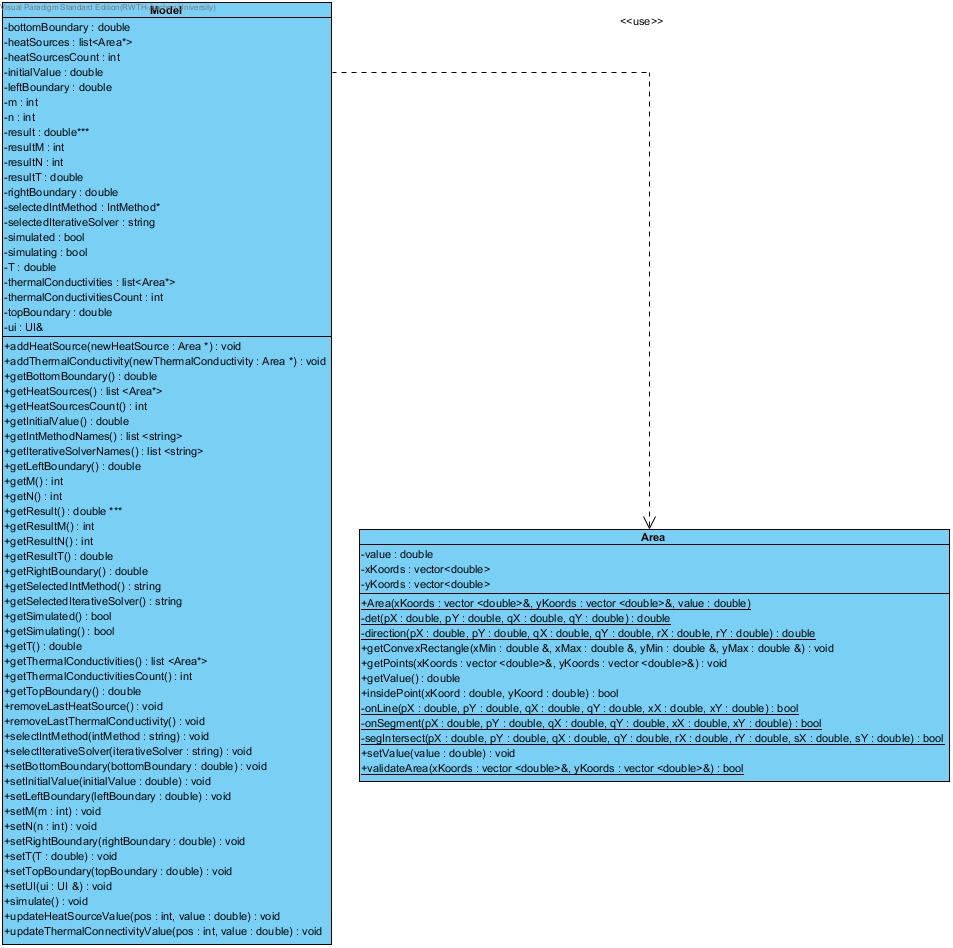
\includegraphics[scale=.6]{Bilder/model.jpg}\\
	\caption{Klassendiagramm model}
	\label{Klassendiagramm model}
\end{figure}

\subsubsection{model}

\subsubsection*{addHeatSource}

Das Sequenzdiagramm für \emph{addHeatSource} ist in \ref{Sequenzdiagramm addHeatSource} dargstellt. \emph{addHeatSource} fügt eine weitere Wärmequelle hinzu.

%Sequenzdiagramm addHeatSource
\begin{figure}[H]
	\centering
	%\hspace{-.5cm}
	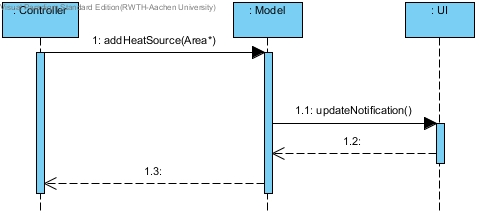
\includegraphics[scale=.6]{Bilder/Model__addHeatSource().jpg}\\
	\caption{Sequenzdiagramm addHeatSource}
	\label{Sequenzdiagramm addHeatSource}
\end{figure}

\subsubsection*{addThermalDiffusivity}

Das Sequenzdiagramm für \emph{addThermalDiffusivity} ist in \ref{Sequenzdiagramm addThermalDiffusivity} dargstellt. \emph{addThermalDiffusivity} fügt ein durch den Nutzer gewähltes Gebiet mit zugehörigem Temperaturleitkoeffizienten hinzu.

%Sequenzdiagramm addThermalDiffusivity
\begin{figure}[H]
	\centering
	%\hspace{-.5cm}
	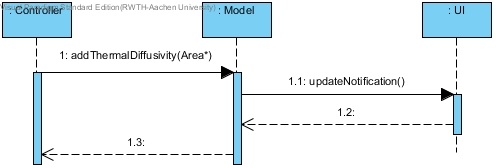
\includegraphics[scale=.6]{Bilder/Model__addThermalDiffusivity().jpg}\\
	\caption{Sequenzdiagramm addThermalDiffusivity}
	\label{Sequenzdiagramm addThermalDiffusivity}
\end{figure}

\subsubsection*{removeLastHeatSource}

Das Sequenzdiagramm für \emph{removeLastHeatSource} ist in \ref{Sequenzdiagramm removeLastHeatSource} dargstellt.

%Sequenzdiagramm removeLastHeatSource
\begin{figure}[H]
	\centering
	%\hspace{-.5cm}
	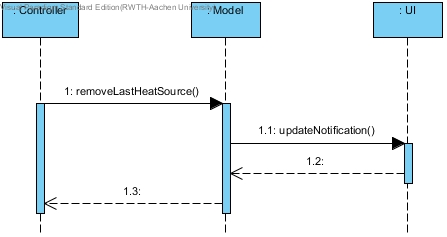
\includegraphics[scale=.6]{Bilder/Model__removeLastHeatSource().jpg}\\
	\caption{Sequenzdiagramm removeLastHeatSource}
	\label{Sequenzdiagramm removeLastHeatSource}
\end{figure}

\subsubsection*{removeLastThermalDiffusivity}

Das Sequenzdiagramm für \emph{removeLastThermalDiffusivity} ist in \ref{Sequenzdiagramm removeLastThermalDiffusivity} dargstellt.

%Sequenzdiagramm removeLastThermalDiffusivity
\begin{figure}[H]
	\centering
	%\hspace{-.5cm}
	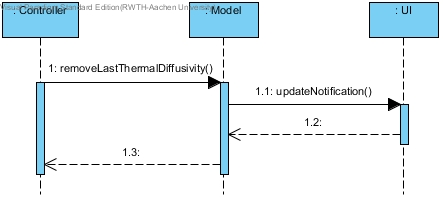
\includegraphics[scale=.6]{Bilder/Model__removeLastThermalDiffusivity().jpg}\\
	\caption{Sequenzdiagramm removeLastThermalDiffusivity}
	\label{Sequenzdiagramm removeLastThermalDiffusivity}
\end{figure}

\subsubsection*{selectIntMethod}

Das Sequenzdiagramm für \emph{selectIntMethod} ist in \ref{Sequenzdiagramm selectIntMethod} dargstellt.

%Sequenzdiagramm selectIntMethod
\begin{figure}[H]
	\centering
	%\hspace{-.5cm}
	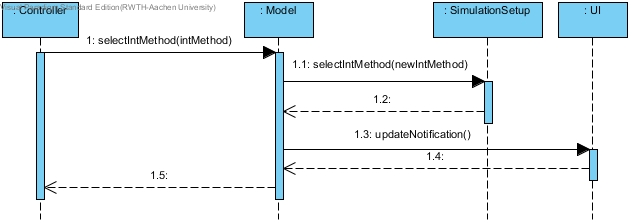
\includegraphics[scale=.6]{Bilder/Model__selectIntMethod().jpg}\\
	\caption{Sequenzdiagramm selectIntMethod}
	\label{Sequenzdiagramm selectIntMethod}
\end{figure}

\subsubsection*{selectSolver}

Das Sequenzdiagramm für \emph{selectSolver} ist in \ref{Sequenzdiagramm selectSolver} dargstellt.

%Sequenzdiagramm selectSolver
\begin{figure}[H]
	\centering
	%\hspace{-.5cm}
	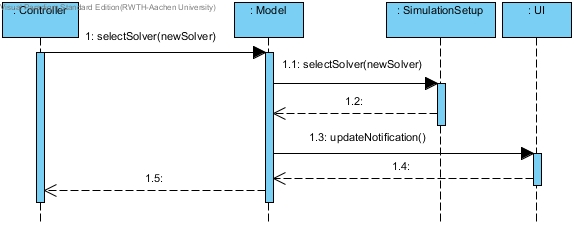
\includegraphics[scale=.6]{Bilder/Model__selectSolver().jpg}\\
	\caption{Sequenzdiagramm selectSolver}
	\label{Sequenzdiagramm selectSolver}
\end{figure}

\subsubsection*{setBottomBoundary}

Das Sequenzdiagramm für \emph{setBottomBoundary} ist in \ref{Sequenzdiagramm setBottomBoundary} dargstellt.

%Sequenzdiagramm setBottomBoundary
\begin{figure}[H]
	\centering
	%\hspace{-.5cm}
	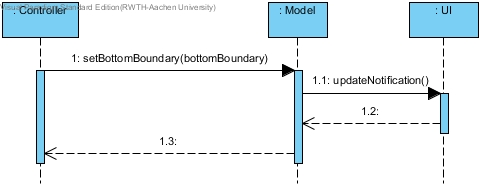
\includegraphics[scale=.6]{Bilder/Model__setBottomBoundary().jpg}\\
	\caption{Sequenzdiagramm setBottomBoundary}
	\label{Sequenzdiagramm setBottomBoundary}
\end{figure}

\subsubsection*{setInitialValue}

Das Sequenzdiagramm für \emph{setInitialValue} ist in \ref{Sequenzdiagramm setInitialValue} dargstellt.

%Sequenzdiagramm setInitialValue
\begin{figure}[H]
	\centering
	%\hspace{-.5cm}
	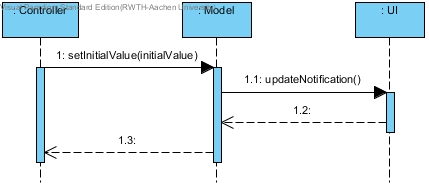
\includegraphics[scale=.6]{Bilder/Model__setInitialValue().jpg}\\
	\caption{Sequenzdiagramm setInitialValue}
	\label{Sequenzdiagramm setInitialValue}
\end{figure}

\subsubsection*{setLeftBoundary}

Das Sequenzdiagramm für \emph{setLeftBoundary} ist in \ref{Sequenzdiagramm setLeftBoundary} dargstellt.

%Sequenzdiagramm setLeftBoundary
\begin{figure}[H]
	\centering
	%\hspace{-.5cm}
	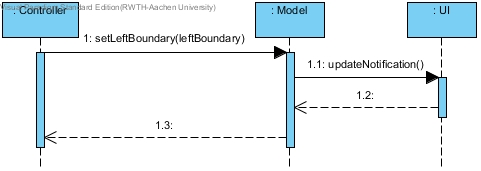
\includegraphics[scale=.6]{Bilder/Model__setLeftBoundary().jpg}\\
	\caption{Sequenzdiagramm setLeftBoundary}
	\label{Sequenzdiagramm setLeftBoundary}
\end{figure}


\subsubsection*{setM}

Das Sequenzdiagramm für \emph{setM} ist in \ref{Sequenzdiagramm setM} dargstellt.

%Sequenzdiagramm setM
\begin{figure}[H]
	\centering
	%\hspace{-.5cm}
	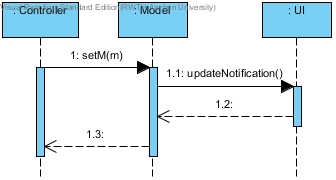
\includegraphics[scale=.6]{Bilder/Model__setM().jpg}\\
	\caption{Sequenzdiagramm setM}
	\label{Sequenzdiagramm setM}
\end{figure}

\subsubsection*{setN}

Das Sequenzdiagramm für \emph{setN} ist in \ref{Sequenzdiagramm setN} dargstellt.

%Sequenzdiagramm setN
\begin{figure}[H]
	\centering
	%\hspace{-.5cm}
	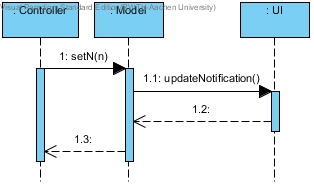
\includegraphics[scale=.6]{Bilder/Model__setN().jpg}\\
	\caption{Sequenzdiagramm setN}
	\label{Sequenzdiagramm setN}
\end{figure}

\subsubsection*{setRightBoundary}

Das Sequenzdiagramm für \emph{setRightBoundary} ist in \ref{Sequenzdiagramm setRightBoundary} dargstellt.

%Sequenzdiagramm setRightBoundary
\begin{figure}[H]
	\centering
	%\hspace{-.5cm}
	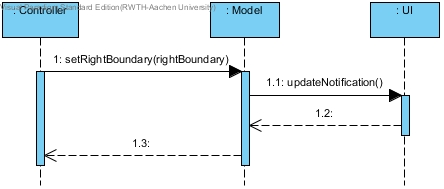
\includegraphics[scale=.6]{Bilder/Model__setRightBoundary().jpg}\\
	\caption{Sequenzdiagramm setRightBoundary}
	\label{Sequenzdiagramm setRightBoundary}
\end{figure}

\subsubsection*{setT}

Das Sequenzdiagramm für \emph{setT} ist in \ref{Sequenzdiagramm setT} dargstellt.

%Sequenzdiagramm setT
\begin{figure}[H]
	\centering
	%\hspace{-.5cm}
	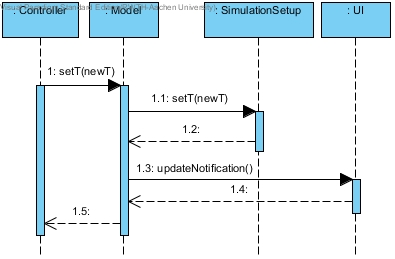
\includegraphics[scale=.6]{Bilder/Model__setT().jpg}\\
	\caption{Sequenzdiagramm setT}
	\label{Sequenzdiagramm setT}
\end{figure}

\subsubsection*{setTopBoundary}

Das Sequenzdiagramm für \emph{setTopBoundary} ist in \ref{Sequenzdiagramm setTopBoundary} dargstellt.

%Sequenzdiagramm setTopBoundary
\begin{figure}[H]
	\centering
	%\hspace{-.5cm}
	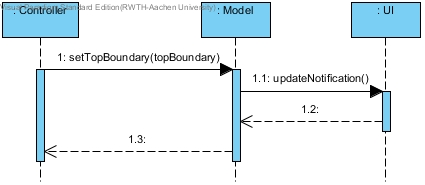
\includegraphics[scale=.6]{Bilder/Model__setTopBoundary().jpg}\\
	\caption{Sequenzdiagramm setTopBoundary}
	\label{Sequenzdiagramm setTopBoundary}
\end{figure}

\subsubsection*{simulate}

Das Sequenzdiagramm für \emph{simulate} ist in \ref{Sequenzdiagramm simulate} dargstellt.

%Sequenzdiagramm simulate
\begin{figure}[H]
	\centering
	%\hspace{-.5cm}
	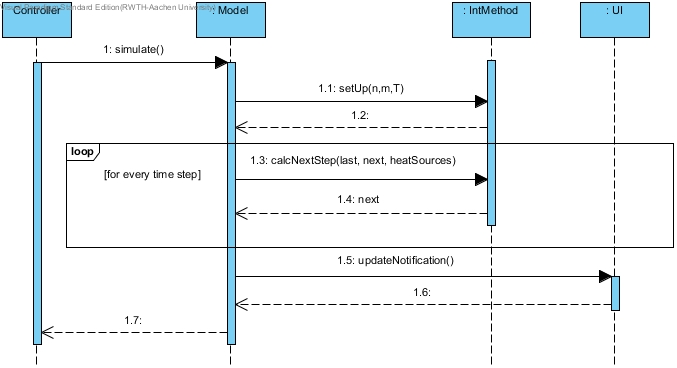
\includegraphics[scale=.6]{Bilder/Model__simulate().jpg}\\
	\caption{Sequenzdiagramm simulate}
	\label{Sequenzdiagramm simulate}
\end{figure}

\subsection{Paket presentation}

Das Klassendiagramm in Abbildung \ref{Klassendiagramm presentation} zeigt alle im Paket \emph{presentation} enthaltene Klassen.

%Klassendiagramm presentation
\begin{figure}[H]
	\centering
	%\hspace{-.5cm}
	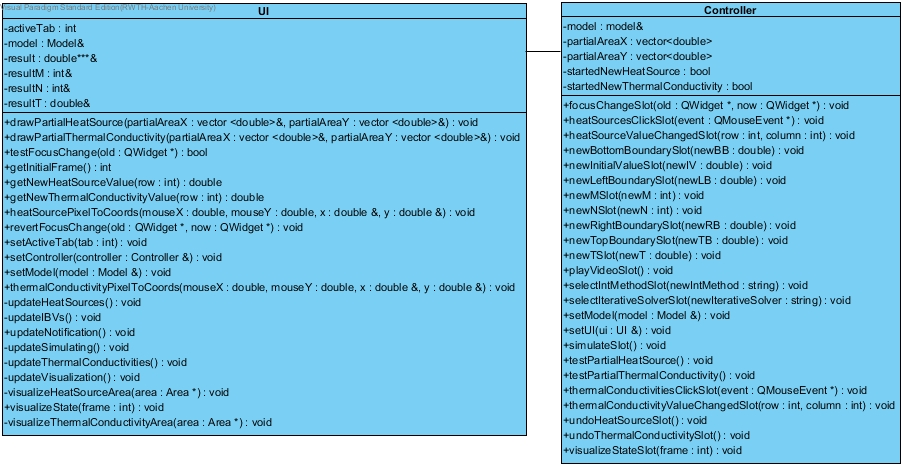
\includegraphics[scale=.9]{Bilder/presentation.jpg}\\
	\caption{Klassendiagramm presentation}
	\label{Klassendiagramm presentation}
\end{figure}

\subsubsection{UI}

Es werden lediglich die Sequenzdiagramme der Update-Methoden dargestellt.

\subsubsection*{updateHeatSources}

Das Sequenzdiagramm für \emph{updateHeatSources} ist in \ref{Sequenzdiagramm updateHeatSources} dargstellt.

%Sequenzdiagramm updateHeatSources
\begin{figure}[H]
	\centering
	%\hspace{-.5cm}
	\includegraphics[scale=.6]{Bilder/UI__updateHeatSources().jpg}\\
	\caption{Sequenzdiagramm updateHeatSources}
	\label{Sequenzdiagramm updateHeatSources}
\end{figure}

\subsubsection*{updateIBVs}

Das Sequenzdiagramm für \emph{updateIBVs} ist in \ref{Sequenzdiagramm updateIBVs} dargstellt.

%Sequenzdiagramm updateIBVs
\begin{figure}[H]
	\centering
	%\hspace{-.5cm}
	\includegraphics[scale=.6]{Bilder/UI__updateIBVs().jpg}\\
	\caption{Sequenzdiagramm updateIBVs}
	\label{Sequenzdiagramm updateIBVs}
\end{figure}

\subsubsection*{updateNotification}

Das Sequenzdiagramm für \emph{updateNotification} ist in \ref{Sequenzdiagramm updateNotification} dargstellt.

%Sequenzdiagramm updateNotification
\begin{figure}[H]
	\centering
	%\hspace{-.5cm}
	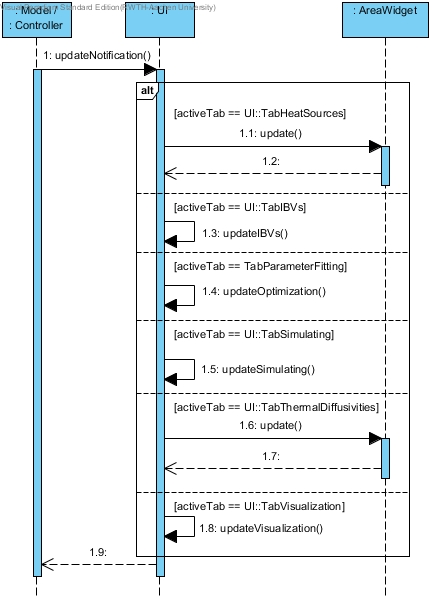
\includegraphics[scale=.6]{Bilder/UI__updateNotification().jpg}\\
	\caption{Sequenzdiagramm updateNotification}
	\label{Sequenzdiagramm updateNotification}
\end{figure}

\subsubsection*{updateSimulating}

Das Sequenzdiagramm für \emph{updateSimulating} ist in \ref{Sequenzdiagramm updateSimulating} dargstellt.

%Sequenzdiagramm updateSimulating
\begin{figure}[H]
	\centering
	%\hspace{-.5cm}
	\includegraphics[scale=.6]{Bilder/UI__updateSimulating().jpg}\\
	\caption{Sequenzdiagramm updateSimulating}
	\label{Sequenzdiagramm updateSimulating}
\end{figure}

\subsubsection*{updateThermalConductivities}

Das Sequenzdiagramm für \emph{updateThermalConductivities} ist in \ref{Sequenzdiagramm updateThermalConductivities} dargstellt.

%Sequenzdiagramm updateThermalConductivities
\begin{figure}[H]
	\centering
	%\hspace{-.5cm}
	\includegraphics[scale=.6]{Bilder/UI__updateThermalConductivities().jpg}\\
	\caption{Sequenzdiagramm updateThermalConductivities}
	\label{Sequenzdiagramm updateThermalConductivities}
\end{figure}

\subsubsection*{updateVisualization}

Das Sequenzdiagramm für \emph{updateVisualization} ist in \ref{Sequenzdiagramm updateVisualization} dargstellt.

%Sequenzdiagramm updateVisualization
\begin{figure}[H]
	\centering
	%\hspace{-.5cm}
	\includegraphics[scale=.6]{Bilder/UI__updateVisualization().jpg}\\
	\caption{Sequenzdiagramm updateVisualization}
	\label{Sequenzdiagramm updateVisualization}
\end{figure}

\subsubsection{Controller}

\subsubsection*{focusChangedSlot}

Das Sequenzdiagramm für \emph{focusChangedSlot} ist in \ref{Sequenzdiagramm focusChangedSlot} dargstellt.

%Sequenzdiagramm focusChangedSlot
\begin{figure}[H]
	\centering
	%\hspace{-.5cm}
	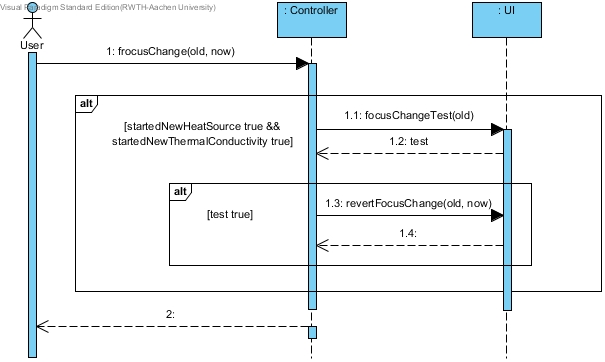
\includegraphics[scale=.6]{Bilder/Controller__focusChangeSlot().jpg}\\
	\caption{Sequenzdiagramm focusChangedSlot}
	\label{Sequenzdiagramm focusChangedSlot}
\end{figure}

\subsubsection*{heatSourceClickSlot}

Das Sequenzdiagramm für \emph{heatSourceClickSlot} ist in \ref{Sequenzdiagramm heatSourceClickSlot} dargstellt.

%Sequenzdiagramm heatSourceClickSlot
\begin{figure}[H]
	\centering
	%\hspace{-.5cm}
	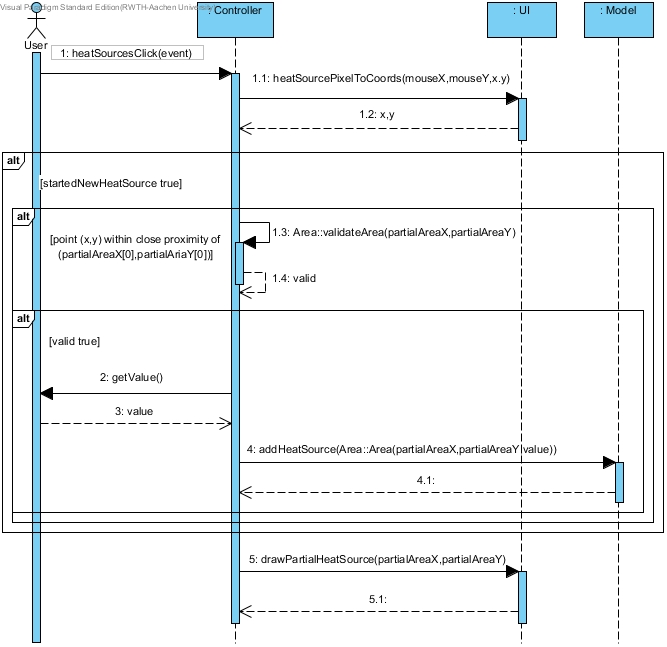
\includegraphics[scale=.6]{Bilder/Controller__heatSourcesClickSlot().jpg}\\
	\caption{Sequenzdiagramm heatSourceClickSlot}
	\label{Sequenzdiagramm heatSourceClickSlot}
\end{figure}

\subsubsection*{newBottomBoundarySlot}

Das Sequenzdiagramm für \emph{newBottomBoundarySlot} ist in \ref{Sequenzdiagramm newBottomBoundarySlot} dargstellt.

%Sequenzdiagramm newBottomBoundarySlot
\begin{figure}[H]
	\centering
	%\hspace{-.5cm}
	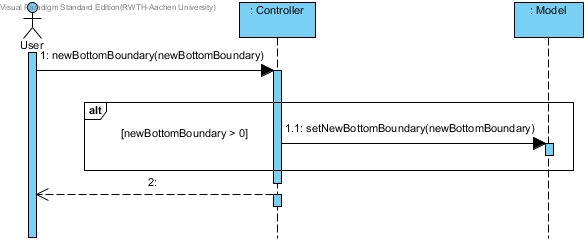
\includegraphics[scale=.6]{Bilder/Controller__newBottomBoundarySlot().jpg}\\
	\caption{Sequenzdiagramm newBottomBoundarySlot}
	\label{Sequenzdiagramm newBottomBoundarySlot}
\end{figure}

\subsubsection*{newInitialValueSlot}

Das Sequenzdiagramm für \emph{newInitialValueSlot} ist in \ref{Sequenzdiagramm newInitialValueSlot} dargstellt.

%Sequenzdiagramm newInitialValueSlot
\begin{figure}[H]
	\centering
	%\hspace{-.5cm}
	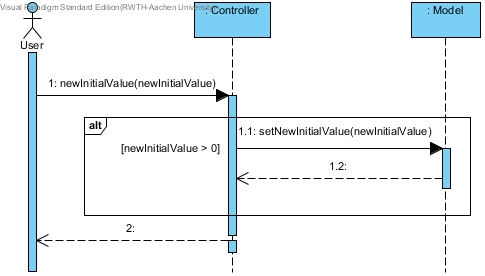
\includegraphics[scale=.6]{Bilder/Controller__newInitialValueSlot().jpg}\\
	\caption{Sequenzdiagramm newInitialValueSlot}
	\label{Sequenzdiagramm newInitialValueSlot}
\end{figure}

\subsubsection*{newInitialValueSlot}

Das Sequenzdiagramm für \emph{newInitialValueSlot} ist in \ref{Sequenzdiagramm newInitialValueSlot} dargstellt.

%Sequenzdiagramm newInitialValueSlot
\begin{figure}[H]
	\centering
	%\hspace{-.5cm}
	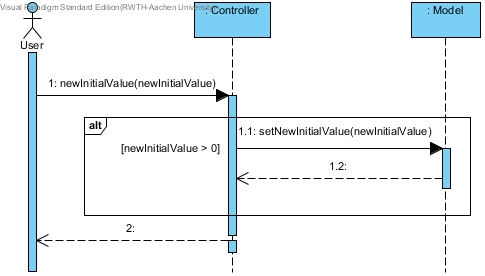
\includegraphics[scale=.6]{Bilder/Controller__newInitialValueSlot().jpg}\\
	\caption{Sequenzdiagramm newInitialValueSlot}
	\label{Sequenzdiagramm newInitialValueSlot}
\end{figure}

\subsubsection*{newLeftBoundarySlot}

Das Sequenzdiagramm für \emph{newLeftBoundarySlot} ist in \ref{Sequenzdiagramm newLeftBoundarySlot} dargstellt.

%Sequenzdiagramm newLeftBoundarySlot
\begin{figure}[H]
	\centering
	%\hspace{-.5cm}
	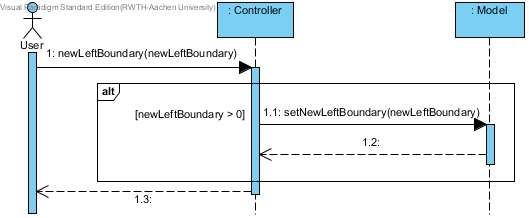
\includegraphics[scale=.6]{Bilder/Controller__newLeftBoundarySlot().jpg}\\
	\caption{Sequenzdiagramm newLeftBoundarySlot}
	\label{Sequenzdiagramm newLeftBoundarySlot}
\end{figure}

\subsubsection*{newMSlot}

Das Sequenzdiagramm für \emph{newMSlot} ist in \ref{Sequenzdiagramm newMSlot} dargstellt.

%Sequenzdiagramm newMSlot
\begin{figure}[H]
	\centering
	%\hspace{-.5cm}
	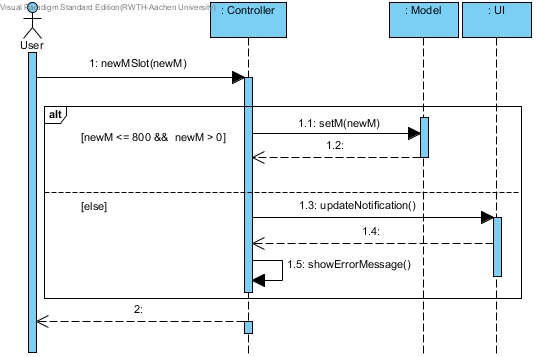
\includegraphics[scale=.6]{Bilder/Controller__newMSlot().jpg}\\
	\caption{Sequenzdiagramm newMSlot}
	\label{Sequenzdiagramm newMSlot}
\end{figure}

\subsubsection*{newNSlot}

Das Sequenzdiagramm für \emph{newNSlot} ist in \ref{Sequenzdiagramm newNSlot} dargstellt.

%Sequenzdiagramm newNSlot
\begin{figure}[H]
	\centering
	%\hspace{-.5cm}
	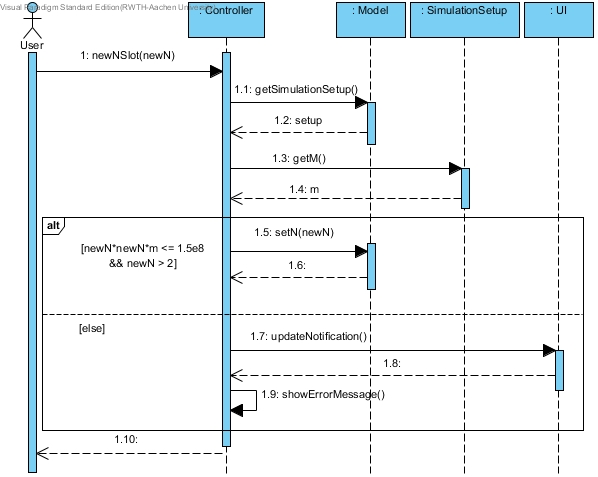
\includegraphics[scale=.6]{Bilder/Controller__newNSlot().jpg}\\
	\caption{Sequenzdiagramm newNSlot}
	\label{Sequenzdiagramm newNSlot}
\end{figure}

\subsubsection*{newRightBoundarySlot}

Das Sequenzdiagramm für \emph{newRightBoundarySlot} ist in \ref{Sequenzdiagramm newRightBoundarySlot} dargstellt.

%Sequenzdiagramm newRightBoundarySlot
\begin{figure}[H]
	\centering
	%\hspace{-.5cm}
	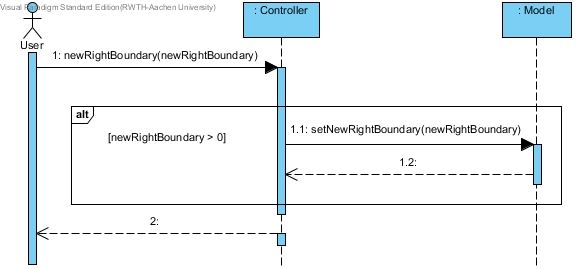
\includegraphics[scale=.6]{Bilder/Controller__newRightBoundarySlot().jpg}\\
	\caption{Sequenzdiagramm newRightBoundarySlot}
	\label{Sequenzdiagramm newRightBoundarySlot}
\end{figure}

\subsubsection*{newTopBoundarySlot}

Das Sequenzdiagramm für \emph{newTopBoundarySlot} ist in \ref{Sequenzdiagramm newTopBoundarySlot} dargstellt.

%Sequenzdiagramm newTopBoundarySlot
\begin{figure}[H]
	\centering
	%\hspace{-.5cm}
	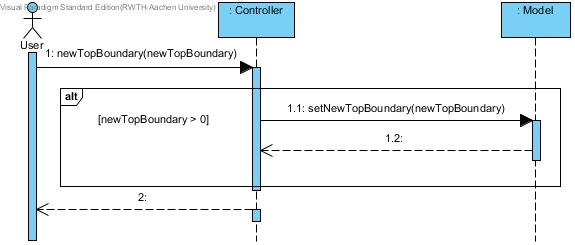
\includegraphics[scale=.6]{Bilder/Controller__newTopBoundarySlot().jpg}\\
	\caption{Sequenzdiagramm newTopBoundarySlot}
	\label{Sequenzdiagramm newTopBoundarySlot}
\end{figure}

\subsubsection*{newTSlot}

Das Sequenzdiagramm für \emph{newTSlot} ist in \ref{Sequenzdiagramm newTSlot} dargstellt.

%Sequenzdiagramm newTSlot
\begin{figure}[H]
	\centering
	%\hspace{-.5cm}
	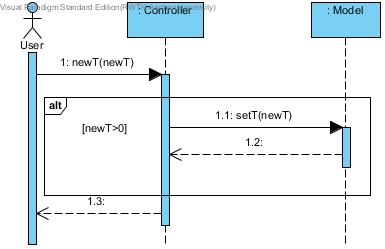
\includegraphics[scale=.6]{Bilder/Controller__newTSlot().jpg}\\
	\caption{Sequenzdiagramm newTSlot}
	\label{Sequenzdiagramm newTSlot}
\end{figure}

\subsubsection*{newTSlot}

Das Sequenzdiagramm für \emph{newTSlot} ist in \ref{Sequenzdiagramm newTSlot} dargstellt.

%Sequenzdiagramm newTSlot
\begin{figure}[H]
	\centering
	%\hspace{-.5cm}
	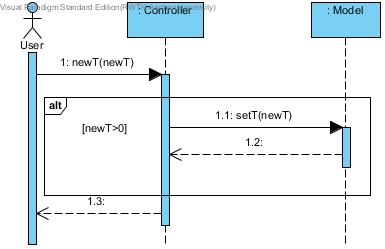
\includegraphics[scale=.6]{Bilder/Controller__newTSlot().jpg}\\
	\caption{Sequenzdiagramm newTSlot}
	\label{Sequenzdiagramm newTSlot}
\end{figure}

\subsubsection*{playVideoSlot}

Das Sequenzdiagramm für \emph{playVideoSlot} ist in \ref{Sequenzdiagramm playVideoSlot} dargstellt.

%Sequenzdiagramm playVideoSlot
\begin{figure}[H]
	\centering
	%\hspace{-.5cm}
	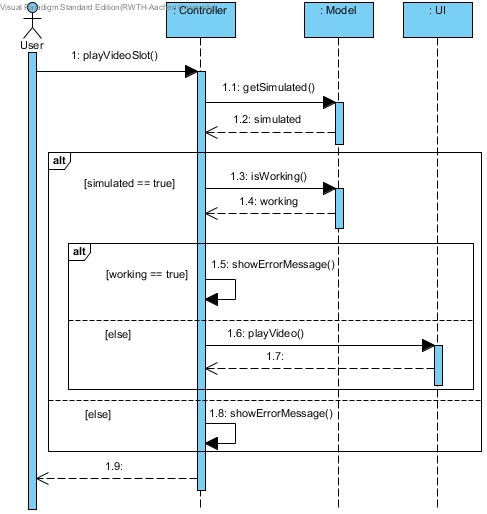
\includegraphics[scale=.6]{Bilder/Controller__playVideoSlot().jpg}\\
	\caption{Sequenzdiagramm playVideoSlot}
	\label{Sequenzdiagramm playVideoSlot}
\end{figure}

\subsubsection*{selectIntMethodSlot}

Das Sequenzdiagramm für \emph{selectIntMethodSlot} ist in \ref{Sequenzdiagramm selectIntMethodSlot} dargstellt.

%Sequenzdiagramm selectIntMethodSlot
\begin{figure}[H]
	\centering
	%\hspace{-.5cm}
	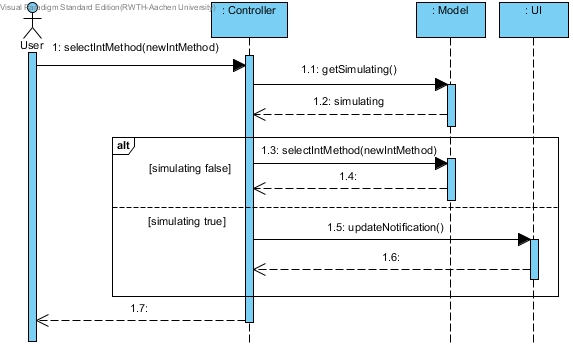
\includegraphics[scale=.6]{Bilder/Controller__selectIntMethodSlot().jpg}\\
	\caption{Sequenzdiagramm selectIntMethodSlot}
	\label{Sequenzdiagramm selectIntMethodSlot}
\end{figure}

\subsubsection*{selectIterativeSolverSlot}

Das Sequenzdiagramm für \emph{selectIterativeSolverSlot} ist in \ref{Sequenzdiagramm selectIterativeSolverSlot} dargstellt.

%Sequenzdiagramm selectIterativeSolverSlot
\begin{figure}[H]
	\centering
	%\hspace{-.5cm}
	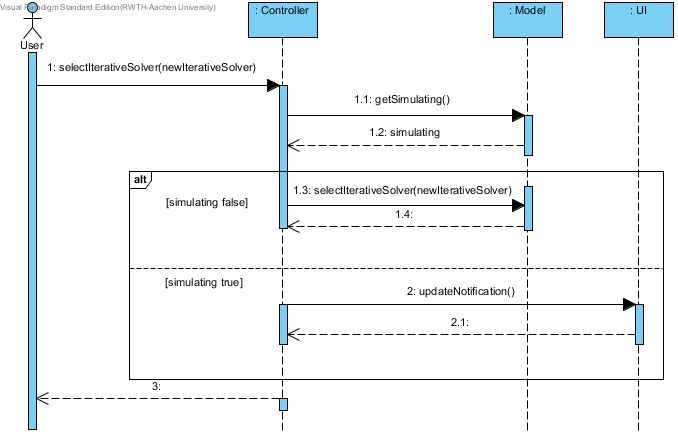
\includegraphics[scale=.6]{Bilder/Controller__selectIterativeSolverSlot().jpg}\\
	\caption{Sequenzdiagramm selectIterativeSolverSlot}
	\label{Sequenzdiagramm selectIterativeSolverSlot}
\end{figure}

\subsubsection*{simulateSlot}

Das Sequenzdiagramm für \emph{simulateSlot} ist in \ref{Sequenzdiagramm simulateSlot} dargstellt.

%Sequenzdiagramm simulateSlot
\begin{figure}[H]
	\centering
	%\hspace{-.5cm}
	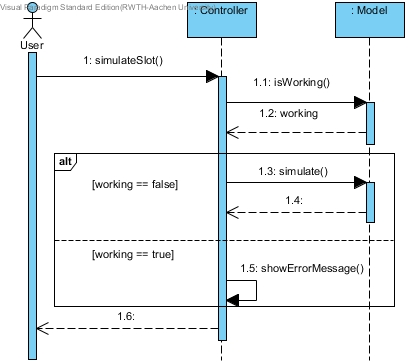
\includegraphics[scale=.6]{Bilder/Controller__simulateSlot().jpg}\\
	\caption{Sequenzdiagramm simulateSlot}
	\label{Sequenzdiagramm simulateSlot}
\end{figure}

\subsubsection*{thermalConductivitiesClickSlot}

Das Sequenzdiagramm für \emph{thermalConductivitiesClickSlot} ist in \ref{Sequenzdiagramm thermalConductivitiesClickSlot} dargstellt.

%Sequenzdiagramm thermalConductivitiesClickSlot
\begin{figure}[H]
	\centering
	%\hspace{-.5cm}
	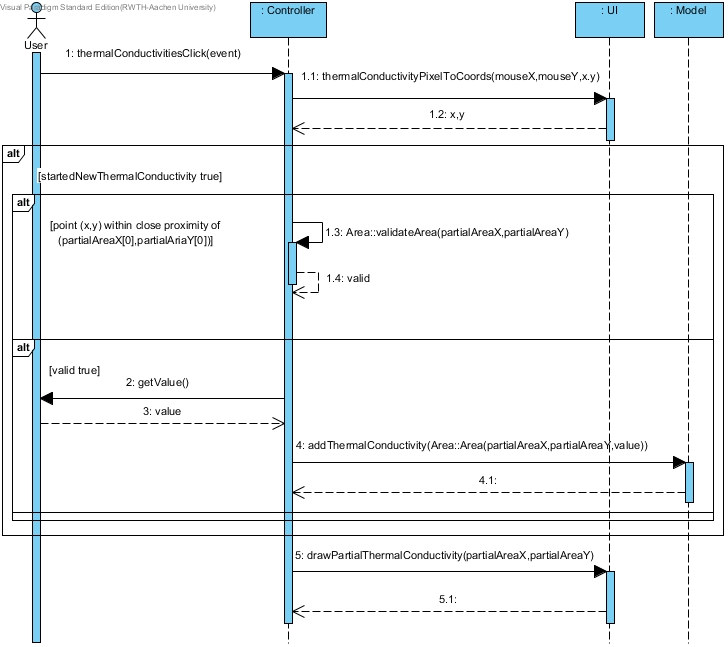
\includegraphics[scale=.6]{Bilder/Controller__thermalConductivitiesClickSlot().jpg}\\
	\caption{Sequenzdiagramm thermalConductivitiesClickSlot}
	\label{Sequenzdiagramm thermalConductivitiesClickSlot}
\end{figure}

\subsubsection*{undoHeatSourceSlot}

Das Sequenzdiagramm für \emph{undoHeatSourceSlot} ist in \ref{Sequenzdiagramm undoHeatSourceSlot} dargstellt.

%Sequenzdiagramm undoHeatSourceSlot
\begin{figure}[H]
	\centering
	%\hspace{-.5cm}
	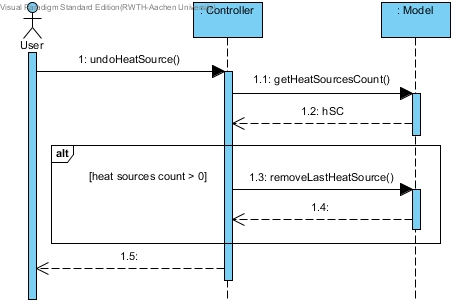
\includegraphics[scale=.6]{Bilder/Controller__undoHeatSourceSlot().jpg}\\
	\caption{Sequenzdiagramm undoHeatSourceSlot}
	\label{Sequenzdiagramm undoHeatSourceSlot}
\end{figure}

\subsubsection*{undoThermalConductivitySlot}

Das Sequenzdiagramm für \emph{undoThermalConductivitySlot} ist in \ref{Sequenzdiagramm undoThermalConductivitySlot} dargstellt.

%Sequenzdiagramm undoThermalConductivitySlot
\begin{figure}[H]
	\centering
	%\hspace{-.5cm}
	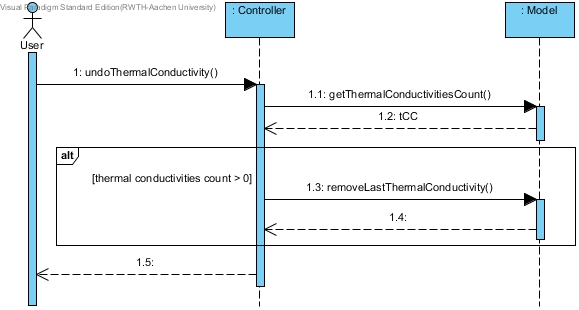
\includegraphics[scale=.6]{Bilder/Controller__undoThermalConductivitySlot().jpg}\\
	\caption{Sequenzdiagramm undoThermalConductivitySlot}
	\label{Sequenzdiagramm undoThermalConductivitySlot}
\end{figure}

\subsubsection*{visualizeStateSlot}

Das Sequenzdiagramm für \emph{visualizeStateSlot} ist in \ref{Sequenzdiagramm visualizeStateSlot} dargstellt.

%Sequenzdiagramm visualizeStateSlot
\begin{figure}[H]
	\centering
	%\hspace{-.5cm}
	\includegraphics[scale=.6]{Bilder/Controller__visualizeStateSlot().jpg}\\
	\caption{Sequenzdiagramm visualizeStateSlot}
	\label{Sequenzdiagramm visualizeStateSlot}
\end{figure}